% 中文版：与 main.tex（英文版）内容逐条对应，数字与结论以 01_diffusion_inverse/results/ 为准。编译：xelatex + bibtex。
\documentclass[11pt,UTF8]{ctexart}
\usepackage[margin=1in]{geometry}
\usepackage{amsmath,amssymb,bm}
\usepackage{booktabs,multirow}
\usepackage{graphicx}
\usepackage{xcolor}
\usepackage{placeins}
\usepackage{hyperref}
\hypersetup{pdftitle={测量应如何进入流匹配 ODE 采样？稀疏视角与低剂量 CT 的对照研究}}
\usepackage[numbers,sort&compress]{natbib}

\newcommand{\A}{\mathcal{A}}
\newcommand{\x}{\bm{x}}
\newcommand{\y}{\bm{y}}
\newcommand{\vel}{\bm{v}_\theta}

\title{测量应如何进入流匹配 ODE 采样？\\稀疏视角与低剂量 CT 的对照研究}
\author{张伟豪\\
  河北大学\\
  \texttt{20268018055@stumail.hbu.edu.cn}}
\date{}

\begin{document}
\maketitle

\begin{abstract}
流匹配先验越来越多地用于 CT 重建，但已发表的方法往往同时改变了先验、网络、数据和测量注入规则，因而很难判断究竟是哪一项在起作用。
本文固定其他一切，只改变测量注入规则。在同一个基于公开 TotalSegmentator CT 数据（1228 例，官方按病人划分）训练的
19.8M 参数 rectified flow 先验上，我们在同一个 Euler ODE 积分器内比较三种规则：梯度引导（DPS 式）、伪逆引导（$\Pi$GDM 式）
和近端数据一致性（DDS/DDNM 式），并与 FBP 以及同骨干的监督网络 FBPConvNet 对比，覆盖 30/60/90 视角稀疏采样与低剂量平行束 CT。
引导强度采用与步数、视角数无关的单位，只在验证集病人上选取；所有比较都给出按病人聚类的 bootstrap 置信区间。主要发现有三点：
(i) 60 视角下伪逆引导的单样本最好（36.9\,dB，比 FBPConvNet 高 1.4\,dB，95\% CI $[0.95,1.91]$）；近端一致性步数效率最高
（20 步即达 36.2\,dB），后验均值也最好（8 个样本时比 FBPConvNet 高 3.9\,dB）。(ii) DPS 式梯度引导在流 ODE 上失效：
无论视角数多少都饱和在约 24.5\,dB，并会产生解剖结构幻觉；初步测量显示其梯度沿轨迹变化约 60 倍。
(iii) 存在光子噪声且没有显式噪声模型时，监督基线仍然更好（$I_0{=}10^5$ 时高 2.2\,dB）；把 $I_0{=}10^5$ 上选出的强度直接
（不重新调参）用于 $I_0{=}10^4$ 时，排名发生倒转。代码、配置与逐图结果已公开。
\end{abstract}

\section{引言}
生成式先验已成为病态 CT 重建中监督后处理之外的有力选择：同一个无条件先验可以复用于不同采集协议，后验采样还能暴露确定性网络
所隐藏的不确定性~\cite{song2022scoremed,chung2022mcg,chung2023dps}。这方面的工作大多基于扩散 SDE。流匹配与
rectified flow~\cite{lipman2023flow,liu2023rectified} 则学习一个速度场，其 ODE 沿近似直线的路径把噪声输运到数据。这使少步采样
很有吸引力，但也改变了测量信息\emph{应在何处}、\emph{以多大强度}注入：ODE 没有逐步重新加噪的过程来吸收引导误差。

流先验用于 CT 是当前的活跃方向~\cite{evangelista2026pgfm,shi2026dm4ct,eFMCT2026,lucid2026}，通用流求解器也以多种方式改造了
扩散引导~\cite{pokle2024otode,martin2025pnpflow,kim2025flowdps}。这些研究大多在改变引导规则的同时也改变了先验、网络、数据或
步长调度；Evangelista~\cite{evangelista2026pgfm} 确实在同一先验（Mayo LDCT）上比较了多个流求解器，但没有采用与步数和视角数无关的
引导强度单位，没有仅用验证集调参，也没有给出按病人的置信区间。引导权重通常依经验选取，而近期工作表明这一选择往往起决定作用
~\cite{moroy2026guidanceweights,barthakur2026leegs}。因此本文只隔离\emph{测量如何进入 ODE} 这一个因素。在 TotalSegmentator
CT~\cite{wasserthal2023totalseg} 上训练的同一个流匹配先验上，我们比较：(M1) 穿过网络的 DPS 式梯度步~\cite{chung2023dps}；
(M2) $\Pi$GDM 式伪逆修正~\cite{song2023pigdm}；(M3) 对预测干净图做共轭梯度近端投影~\cite{chung2024dds}。三者共享先验、积分器、
网络函数评估次数（NFE）、基于验证集的调参协议和测试集，并与 FBP 以及同骨干的监督 FBPConvNet~\cite{jin2017fbpconvnet} 对比。

\paragraph{贡献。}
\begin{itemize}
  \item 在公开数据上、共享 rectified flow 先验的条件下，对稀疏视角（30/60/90）与低剂量 CT 的三种测量注入规则做对照比较，
        仅用验证集调参，并给出按病人的 bootstrap 区间（表~\ref{tab:main}、表~\ref{tab:mean}）。
  \item 使引导强度在不同 NFE、不同视角数之间可比的单位约定：DPS 步长乘以 $\Delta t$ 并除以 $\sqrt{s_x}$，近端权重以 $s_x$ 为单位
        （$s_x=\operatorname{tr}(\A^\top\A)/N^2$，见第 3.3 节）；否则 NFE 消融与跨协议比较会被混淆。
  \item 证据表明梯度引导在流 ODE 上无法利用更多视角（结果不随视角数变化，并有初步测量显示引导梯度沿轨迹变化约 60 倍）；
        伪逆规则与近端规则的不确定性表现不同，使二者在单样本和后验均值上的排名相反。
\end{itemize}

\section{相关工作}
\paragraph{扩散后验采样。}
DPS~\cite{chung2023dps} 和 MCG~\cite{chung2022mcg} 把测量损失穿过去噪网络反传；$\Pi$GDM~\cite{song2023pigdm} 在 $p(\x_0\mid\x_t)$
的高斯近似下用伪逆修正代替梯度；DiffPIR~\cite{zhu2023diffpir}、DDS~\cite{chung2024dds} 和 DAPS~\cite{zhang2025daps} 在去噪与近端 /
数据一致性步之间交替；RED-diff~\cite{mardani2024reddiff} 把采样视为变分优化。针对 CT，基于分数的先验~\cite{song2022scoremed}、
DiffusionMBIR~\cite{chung2023diffusionmbir}、DiffusionBlend~\cite{song2024diffusionblend} 和 DOLCE~\cite{liu2023dolce} 分别处理稀疏视角、
三维与限角问题。DM4CT~\cite{shi2026dm4ct} 对十种扩散方法做了 CT 基准测试；本文与之互补：固定一个流先验，只改变注入规则。
\paragraph{流先验用于反问题与 CT。}
OT-ODE~\cite{pokle2024otode} 为条件 OT 路径推导了类 $\Pi$GDM 修正；PnP-Flow~\cite{martin2025pnpflow} 在流去噪与即插即用投影之间交替；
FlowDPS~\cite{kim2025flowdps} 把流更新分解为干净图与噪声两部分。CT 方面，Evangelista~\cite{evangelista2026pgfm} 在 Mayo LDCT 上训练
rectified flow 先验，并与扩散基线比较了多个流求解器；EFMCT~\cite{eFMCT2026} 在数据一致性中跨步复用速度场；LUCID~\cite{lucid2026}
按稀疏程度调整轨迹并在投影域做修正。引导权重的选取近期有离线最小二乘~\cite{moroy2026guidanceweights} 和学习式调度
~\cite{barthakur2026leegs,bang2026trips} 两类方法。本文的范围不同：单一先验、三种注入规则、与步数和视角无关的单位、
公开数据上仅用验证集调参，以及按病人的统计。
\paragraph{监督 CT 重建。}
FBPConvNet~\cite{jin2017fbpconvnet} 与 LEARN~\cite{chen2018learn} 学习从欠采样数据到图像的映射；它们在分布内很强，但每个协议都要重训。

\section{方法}
\subsection{成像模型}
轴位切片 $\x\in[-1,1]^{N\times N}$（$N{=}256$，HU 窗 $[-1000,1000]$）映射为衰减 $u = m\odot(\x+1)/2$，$m$ 为内切圆掩码。平行束投影
$R_\Theta$ 在 $[0,\pi)$ 内取 $|\Theta|$ 个等距角度；前向模型对 $\x$ 是仿射的：
\begin{equation}
  \A(\x) = R_\Theta(u) = \A_{\mathrm{lin}}\x + \bm{b},\qquad \A_{\mathrm{lin}}\x = R_\Theta(m\odot\x/2),\quad \bm b = R_\Theta(m/2).
\end{equation}
$R_\Theta$ 用双线性插值旋转后求和实现，精确伴随由自动微分得到（伴随相对误差 $<10^{-4}$，有单元测试）。稀疏视角取
$|\Theta|\in\{30,60,90\}$（全采样为 180）。低剂量取 180 视角，加 Poisson 计数噪声 $I\sim\mathrm{Poisson}(I_0 e^{-\mu y})$，
$\y=-\log(I/I_0)/\mu$，$\mu{=}0.06$；主设置为 $I_0{=}10^5$，$I_0{=}10^4$ 作为光子饥饿的极端情形。第 $i$ 张测试图的测量噪声由以
(seed, $i$) 为种子的生成器产生，因此无论 batch 大小、NFE 或后验采样次数如何，所有方法看到的 $\y$ \emph{完全相同}。

\subsection{流匹配先验}
令 $\x_t=(1-t)\bm\epsilon+t\x$，$\bm\epsilon\sim\mathcal N(0,I)$，速度网络最小化 $\mathbb E\|\vel(\x_t,t)-(\x-\bm\epsilon)\|^2$，
$t$ 服从 logit-normal 分布~\cite{esser2024sd3}。由任意状态可读出干净图与噪声的预测
\begin{equation}
  \hat\x_1 = \x_t + (1-t)\,\vel(\x_t,t),\qquad \hat{\bm\epsilon} = \x_t - t\,\vel(\x_t,t).
\end{equation}
无引导采样用步长 $\Delta t = 1/\mathrm{NFE}$ 的 Euler 法把 $\dot\x=\vel$ 从 $t{=}0$ 积分到 $1$。

\subsection{三种测量注入规则}
所有规则都修改同一个 Euler 更新 $\x\leftarrow\x+\Delta t\,\vel$。记 $\bm r=\y-\A(\hat\x_1)$，
$s_x=\operatorname{tr}(\A_{\mathrm{lin}}^\top\A_{\mathrm{lin}})/N^2$，$s_y=\operatorname{tr}(\A_{\mathrm{lin}}\A_{\mathrm{lin}}^\top)/M$（$M$ 为测量数），
二者对每个算子用 16 个高斯探针估计一次。

\paragraph{M1：梯度引导（DPS 式）。}
\begin{equation}
  \x_{t+\Delta t} = \x_t + \Delta t\,\Big(\vel - \frac{\zeta}{\sqrt{s_x}}\,\nabla_{\x_t}\|\A(\hat\x_1)-\y\|_2\Big)\quad (t\ge t_s).
\end{equation}
与 DPS 一致，使用残差\emph{范数}的梯度。与常见实现不同，引导乘以 $\Delta t$，使积分后的总引导量与 NFE 无关（否则 NFE 消融会悄悄改变
$\zeta$ 的实际大小）；并除以 $\sqrt{s_x}$，使 $\zeta$ 在不同视角数下可比。由于梯度范数沿轨迹变化很大（见第 5 节"梯度引导为何失效"），
我们额外调节引导起始时刻 $t_s$。

\paragraph{M2：伪逆引导（$\Pi$GDM 式）。}
在 $\hat\x_1\mid\x_t\sim\mathcal N(\hat\x_1, r_t^2 I)$、$r_t^2=(1-t)^2/(t^2+(1-t)^2)$（$\Pi$GDM 方差在流上的对应）的假设下，在测量空间用
$K{=}5$ 次共轭梯度迭代求解
\begin{equation}
  \big(\A_{\mathrm{lin}}\A_{\mathrm{lin}}^\top + (\sigma_y^2/r_t^2 + \eta\, s_y) I\big)\bm z = \bm r ,
\end{equation}
其中 $\eta{=}10^{-3}$、$\sigma_y{=}0$，再穿过网络做向量--雅可比积：
\begin{equation}
  \x_{t+\Delta t} = \x_t + \Delta t\,\vel + \zeta\, t_{+}\,\Big(\tfrac{\partial\hat\x_1}{\partial\x_t}\Big)^{\!\top}\A_{\mathrm{lin}}^\top\bm z ,
\end{equation}
其中 $t_{+}=t+\Delta t$ 对应 $\Pi$GDM 中的信号系数 $\sqrt{\bar\alpha_t}$。

\paragraph{M3：近端数据一致性（DDS/DDNM 式）。}
把预测干净图替换为
\begin{equation}
  \hat\x_1^{\mathrm{dc}}=\arg\min_{\x}\|\A(\x)-\y\|_2^2+\lambda\|\x-\hat\x_1\|_2^2,\qquad \lambda = \tilde\lambda\, s_x ,
\end{equation}
用 $K{=}5$ 次 CG 求解，再重组状态 $\x_{t+\Delta t}=(1-t_{+})\hat{\bm\epsilon}+t_{+}\hat\x_1^{\mathrm{dc}}$。M3 不需要穿过网络反传。

\section{实验设置}
\paragraph{数据。}
TotalSegmentator v2.0.1~\cite{wasserthal2023totalseg}（1228 例 CT，1.5\,mm 各向同性），取自 Hugging Face 上 CC-BY-4.0 协议的
重新打包版本（\nolinkurl{YongchengYAO/TotalSegmentator-CT-Lite}，压缩包已对照其公布的 SHA-256 校验），采用官方按病人划分。每例最多
沿 $z$ 均匀取 40 张身体占比超过 10\% 的轴位切片，中心裁剪到 $256^2$：训练 43{,}220 张（1082 位病人），验证 2{,}280 张（57 位），测试
3{,}560 张（89 位）。固定测试集 \emph{test200} 为 20 位测试病人 $\times$ 10 张。引导强度只在均匀分布于验证病人的 50 张验证切片上选取，
从不使用测试数据。

\paragraph{先验与基线。}
先验为 19.8M 参数的 U-Net（基础宽度 64，通道倍数 1、1、2、2、4，每层两个残差块，$16^2$ 处自注意力），训练 12 万步，batch 32，
AdamW（学习率 $2{\times}10^{-4}$，1k 步预热，余弦衰减到 $10^{-5}$），EMA 0.9995，bf16 自动混合精度。FBPConvNet 使用\emph{相同}骨干
（$t{\equiv}0$），在 FBP 结果上预测残差，每个协议单独训练 1 万步（batch 16，余弦调度），约 3.7 个 epoch，而先验约 89 个 epoch，
因此其数字应视为下界。FBP 使用 Ram--Lak 滤波，并在均匀圆盘上做一次幅值标定。

\paragraph{调参协议。}
网格（验证集 PSNR，NFE 50）：
\begin{itemize}
  \item M1：60 视角 $\zeta\in\{3,10,30,100,300\}\times t_s\in\{0.1,0.2,0.3,0.4,0.5\}$；$I_0{=}10^5$ 时
        $\zeta\in\{10,30,100\}\times t_s\in\{0.2,\dots,0.5\}$；
  \item M2：$\zeta\in\{0.5,1,2\}$（60 视角），$\zeta\in\{0.03,0.05,0.1,0.25,0.5,1\}$（$I_0{=}10^5$）；
  \item M3：$\tilde\lambda\in\{0.01,0.03,0.1,0.3,1,3\}$（60 视角），$\tilde\lambda\in\{1,3,10,30,100\}$（$I_0{=}10^5$）。
\end{itemize}
网格持续外扩，直到没有最优值落在边界上（共外扩两次）。60 视角选出的参数复用于 30 与 90 视角，$I_0{=}10^5$ 选出的参数用于
$I_0{=}10^4$。选定值：M1 $(\zeta,t_s)=(30,0.4)$（两种情形相同），M2 $\zeta=1$（稀疏）/ $0.1$（低剂量），M3 $\tilde\lambda=0.3$（稀疏）/
$30$（低剂量）。$I_0{=}10^4$ \emph{没有}重新调参。

\paragraph{指标。}
重建圆内的 PSNR（动态范围 2，即 $[-1000,1000]$ HU 窗）；在重建圆内平均的 SSIM（在恒定背景上计算会抬高所有方法）；
LPIPS（AlexNet）~\cite{zhang2018lpips}；测量一致性 $\|\A(\hat\x)-\y\|/\|\y\|$。对生成式方法还报告 $K$ 个样本后验均值的 PSNR
与逐像素后验标准差的均值。由于 200 张测试切片来自 20 位病人，95\% 置信区间与配对差都用按病人的聚类 bootstrap（2000 次重采样）计算。

\paragraph{算力。}
全部实验在单张 RTX~5090（32\,GB）上完成。先验在 \texttt{torch.compile} 与 channels-last 内存布局下为 0.19\,s/步（共 6.3\,h）；
调参与后验采样 3.9\,h，四个 FBPConvNet 共 1.8\,h，合计约 12 GPU 小时。

\section{结果}
\begin{table}[t]
\centering
\caption{test200 上的单样本结果（NFE 50）。PSNR 单位 dB，括号内为按病人的 95\% bootstrap 置信区间；SSIM 在重建圆内计算；
DC $=\|\A(\hat\x)-\y\|/\|\y\|$。每个设置的最佳 PSNR 加粗。}
\label{tab:main}
\small
\begin{tabular}{llcccc}
\toprule
设置 & 方法 & PSNR$\uparrow$ [95\% CI] & SSIM$\uparrow$ & LPIPS$\downarrow$ & DC$\downarrow$ \\
\midrule
\multirow{5}{*}{30 视角} & FBP & 23.50\,{\scriptsize[22.62,24.31]} & 0.429 & 0.365 & 0.0616 \\
 & FBPConvNet（监督） & \textbf{32.22}\,{\scriptsize[30.85,33.54]} & 0.824 & 0.116 & 0.0078 \\
 & M1 梯度引导 & 24.40\,{\scriptsize[23.62,25.07]} & 0.575 & 0.335 & 0.0382 \\
 & M2 $\Pi$GDM 伪逆 & 32.17\,{\scriptsize[30.41,33.90]} & 0.804 & 0.140 & 0.0019 \\
 & M3 近端一致性 & 31.62\,{\scriptsize[29.76,33.31]} & 0.758 & 0.132 & 0.0015 \\
\midrule
\multirow{5}{*}{60 视角} & FBP & 28.50\,{\scriptsize[27.49,29.37]} & 0.635 & 0.222 & 0.0399 \\
 & FBPConvNet（监督） & 35.50\,{\scriptsize[33.83,36.98]} & 0.893 & 0.084 & 0.0050 \\
 & M1 梯度引导 & 24.54\,{\scriptsize[23.78,25.24]} & 0.585 & 0.334 & 0.0387 \\
 & M2 $\Pi$GDM 伪逆 & \textbf{36.93}\,{\scriptsize[34.97,38.74]} & 0.899 & 0.109 & 0.0024 \\
 & M3 近端一致性 & 35.95\,{\scriptsize[33.65,38.28]} & 0.861 & 0.083 & 0.0011 \\
\midrule
\multirow{5}{*}{90 视角} & FBP & 30.58\,{\scriptsize[29.66,31.48]} & 0.734 & 0.143 & 0.0358 \\
 & FBPConvNet（监督） & 37.41\,{\scriptsize[35.63,39.03]} & 0.921 & 0.066 & 0.0045 \\
 & M1 梯度引导 & 24.54\,{\scriptsize[23.78,25.24]} & 0.585 & 0.334 & 0.0389 \\
 & M2 $\Pi$GDM 伪逆 & 38.09\,{\scriptsize[35.97,39.91]} & 0.916 & 0.107 & 0.0032 \\
 & M3 近端一致性 & \textbf{38.62}\,{\scriptsize[35.94,41.11]} & 0.904 & 0.065 & 0.0010 \\
\midrule
\multirow{5}{*}{低剂量 $I_0{=}10^5$} & FBP & 26.21\,{\scriptsize[25.31,26.96]} & 0.580 & 0.309 & 0.0360 \\
 & FBPConvNet（监督） & \textbf{35.32}\,{\scriptsize[33.88,36.51]} & 0.888 & 0.088 & 0.0109 \\
 & M1 梯度引导 & 24.55\,{\scriptsize[23.81,25.25]} & 0.590 & 0.333 & 0.0393 \\
 & M2 $\Pi$GDM 伪逆 & 33.16\,{\scriptsize[31.69,34.48]} & 0.837 & 0.122 & 0.0124 \\
 & M3 近端一致性 & 30.60\,{\scriptsize[29.34,31.88]} & 0.744 & 0.191 & 0.0089 \\
\bottomrule
\end{tabular}

\end{table}

\paragraph{主要比较。}
表~\ref{tab:main} 汇总了单样本结果。两种强制一致性的规则（M2、M3）在稀疏视角下比 FBP 高 7.4--8.7\,dB。与按协议单独训练的监督基线
相比，$\Pi$GDM 在 30 视角持平（$-0.06$\,dB，CI $[-0.69,0.58]$），在 60 视角更好（$+1.43$，$[0.95,1.91]$），90 视角也更好
（$+0.68$，$[0.30,1.04]$）；近端一致性在 90 视角更好（$+1.21$，$[0.18,2.35]$）。两种规则之间，$\Pi$GDM 在 60 视角胜出
（$+0.97$，$[0.35,1.55]$），30 与 90 视角下差异不显著。二者的数据一致性残差为 $0.10$--$0.32\%$，比 FBPConvNet（$0.45$--$0.78\%$）
低数倍。（表~\ref{tab:main} 中 M1 的 60 与 90 视角两行并非复制错误：逐图 PSNR 平均只差 $0.0003$\,dB。）在图~\ref{fig:qual} 的胸部切片上，
FBPConvNet 过度平滑，30 视角下残留条纹；$\Pi$GDM 最锐利；M3 保留了（本身含噪的）真值扫描的噪声纹理。

\begin{figure}[t]
\centering
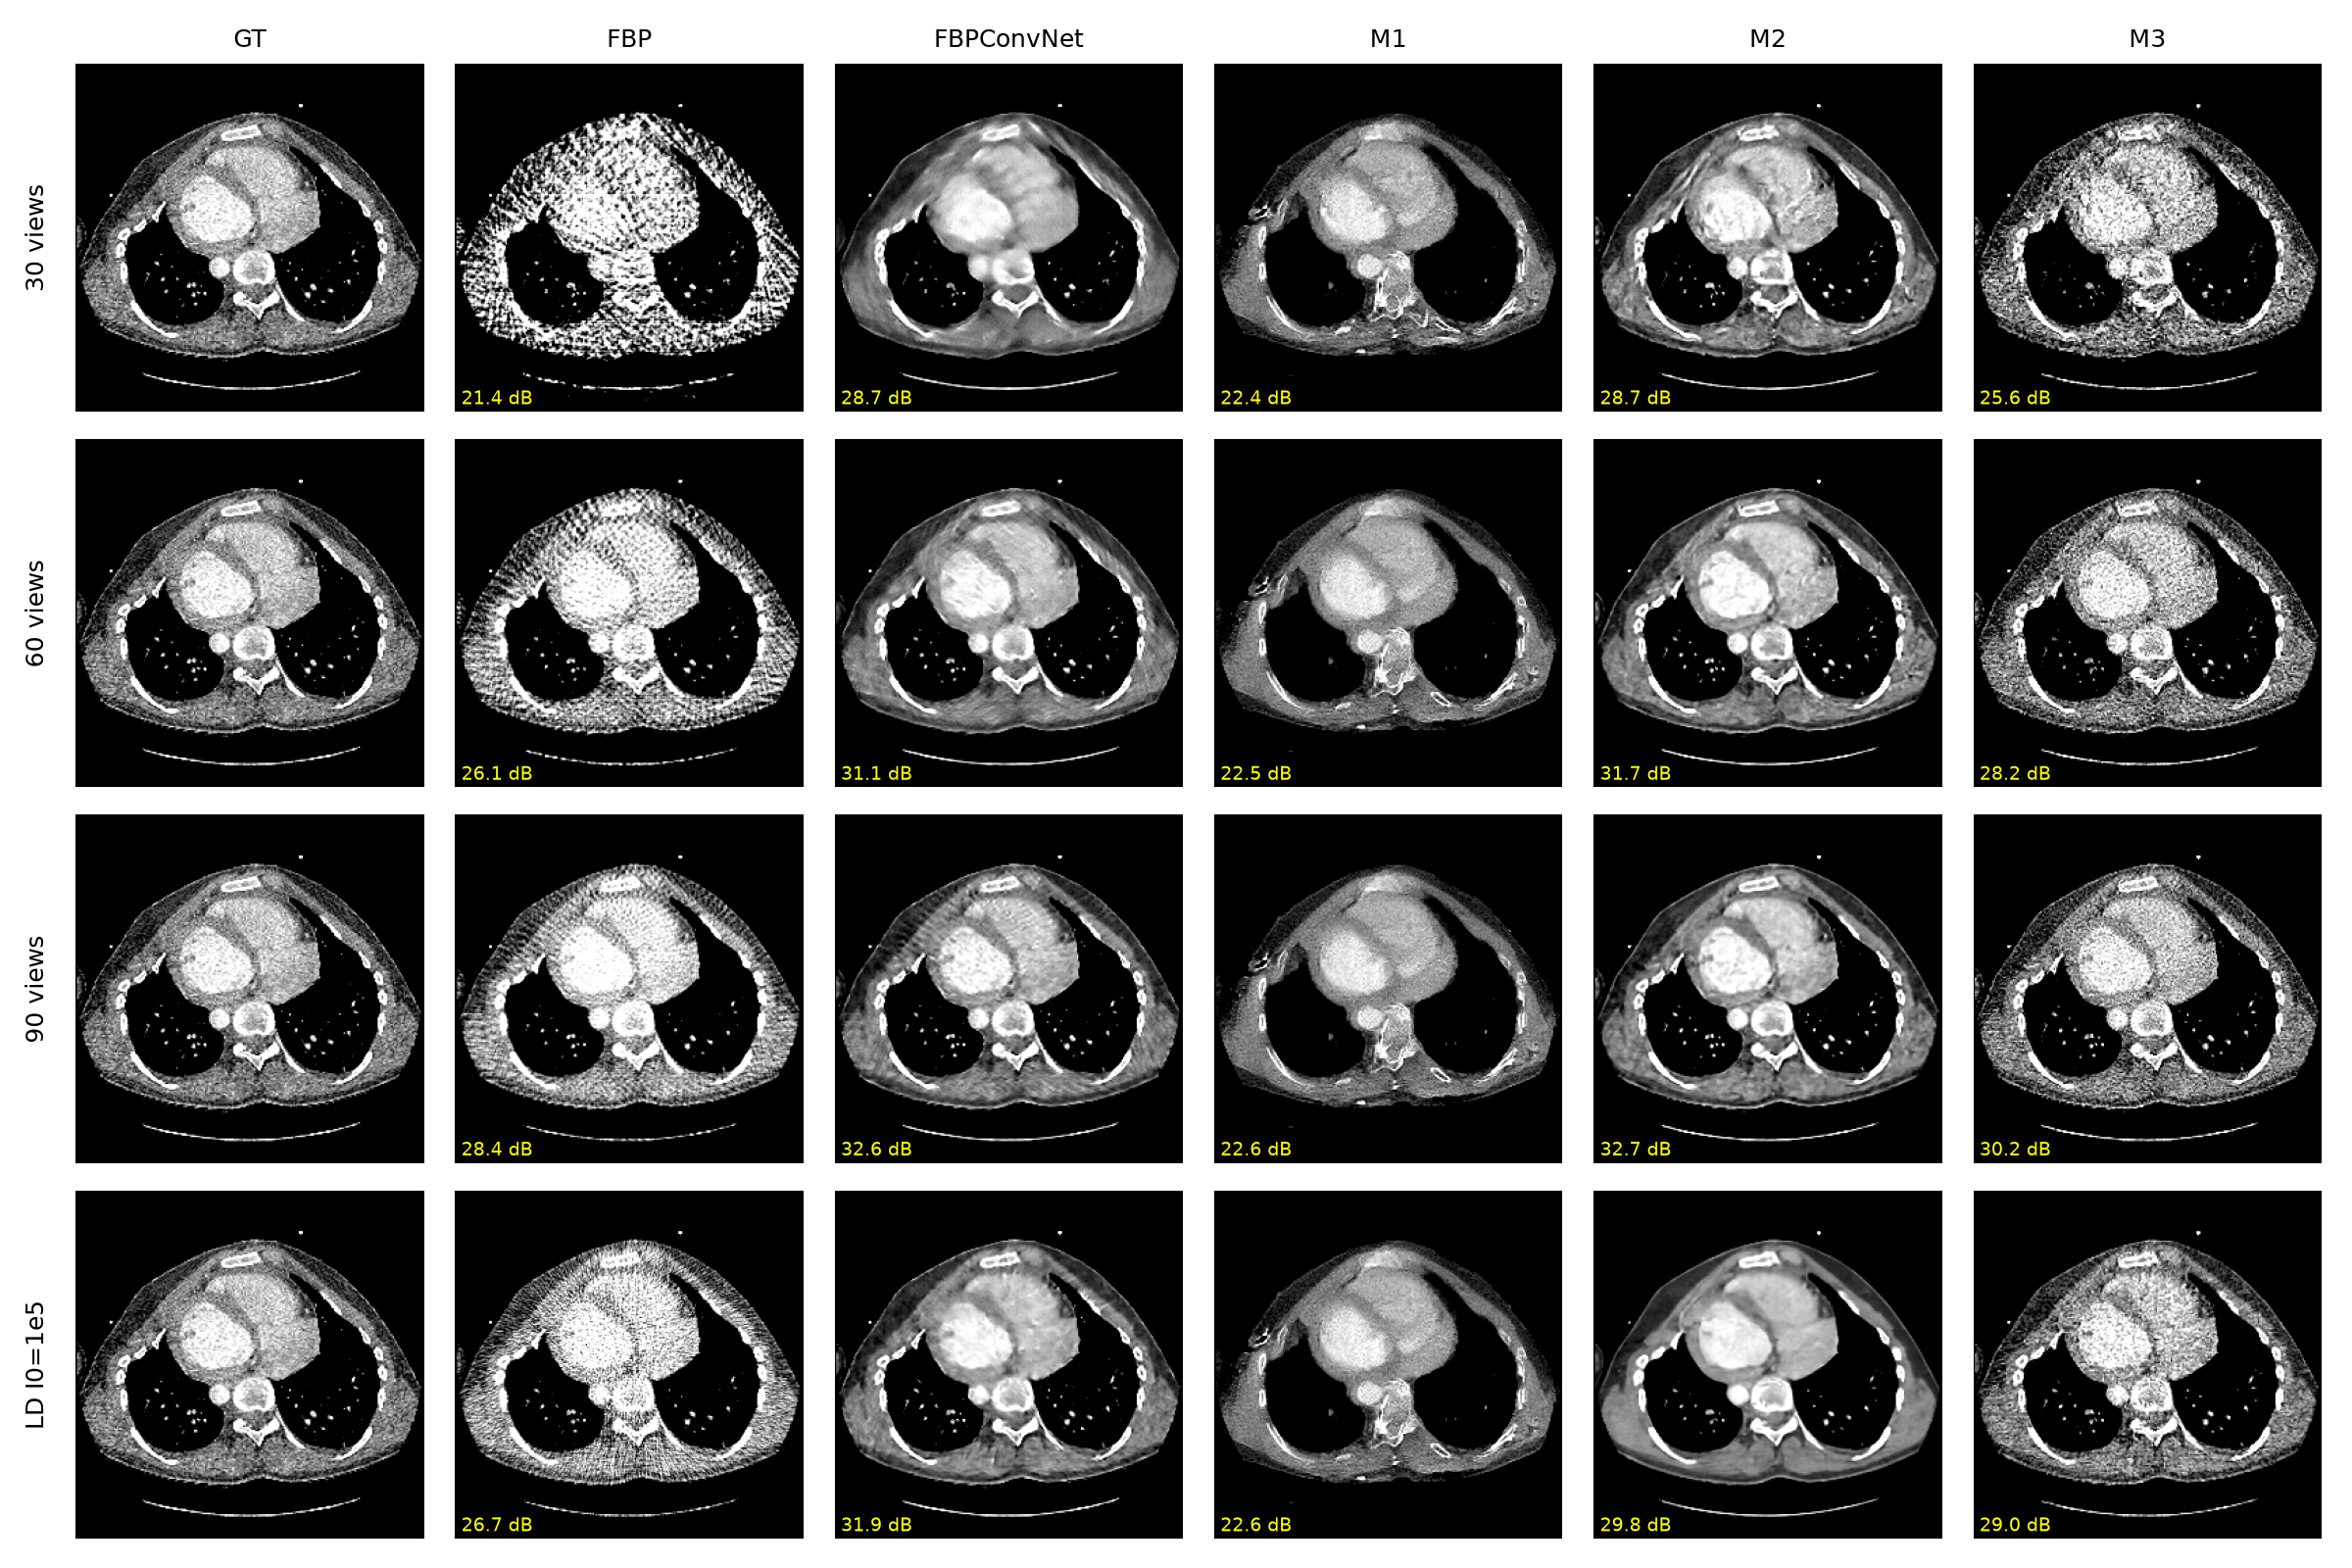
\includegraphics[width=\linewidth]{figures/qualitative.png}
\caption{一张胸部测试切片（软组织窗 W400/L40；重建圆外已遮掉）。数字为圆内 PSNR；这张临床扫描噪声较大，低于数据集平均水平
（见表~\ref{tab:main}）。M1 改变了椎体与肋骨（幻觉）；FBPConvNet 过度平滑；M2 最锐利；M3 保留了测量扫描的噪声纹理。}
\label{fig:qual}
\end{figure}

\paragraph{后验均值使排名反转。}
\begin{table}[t]
\centering
\caption{单样本与 $K$ 个样本后验均值的 PSNR（test200，NFE 50）以及逐像素后验标准差的均值。带置信区间的配对差见正文。}
\label{tab:mean}
\small
\begin{tabular}{llccc}
\toprule
设置 & 方法 & 单样本 & $K$ 样本均值 & 标准差 \\
\midrule
\multirow{3}{*}{60 视角，$K{=}8$} & M1 梯度引导 & 24.53 & 26.22 & 0.129 \\
 & M2 $\Pi$GDM 伪逆 & 36.75 & 38.60 & 0.053 \\
 & M3 近端一致性 & 35.95 & \textbf{39.41} & 0.060 \\
\midrule
\multirow{3}{*}{30 视角，$K{=}4$} & M1 梯度引导 & 24.50 & 25.86 & 0.123 \\
 & M2 $\Pi$GDM 伪逆 & 31.45 & 33.33 & 0.067 \\
 & M3 近端一致性 & 31.63 & \textbf{34.54} & 0.066 \\
\bottomrule
\end{tabular}
\end{table}
对后验样本取平均（表~\ref{tab:mean}）对所有方法都有帮助，但幅度不同：M3 提升 3.5\,dB 并反超 M2，M2 提升 1.9\,dB（后验均值上
M3$-$M2：60 视角 $+0.82$ $[0.28,1.43]$，30 视角 $+1.21$ $[0.43,2.04]$）。后验标准差图（图~\ref{fig:unc}）提示了原因：M2 的不确定性小，
集中在边缘和肺纹理；M3 的不确定性弥散、呈噪声状而非集中于边缘，这与"样本主要在测量未约束的分量上不同、平均后相互抵消"一致。
与监督网络相比，M3 后验均值高 2.3--3.9\,dB（30 视角 $[1.65,3.02]$，60 视角 $[2.97,4.95]$），M2 后验均值高 1.1--3.1\,dB。
因此，输出取单样本还是后验均值，决定了哪种规则更可取。

\begin{figure}[t]
\centering
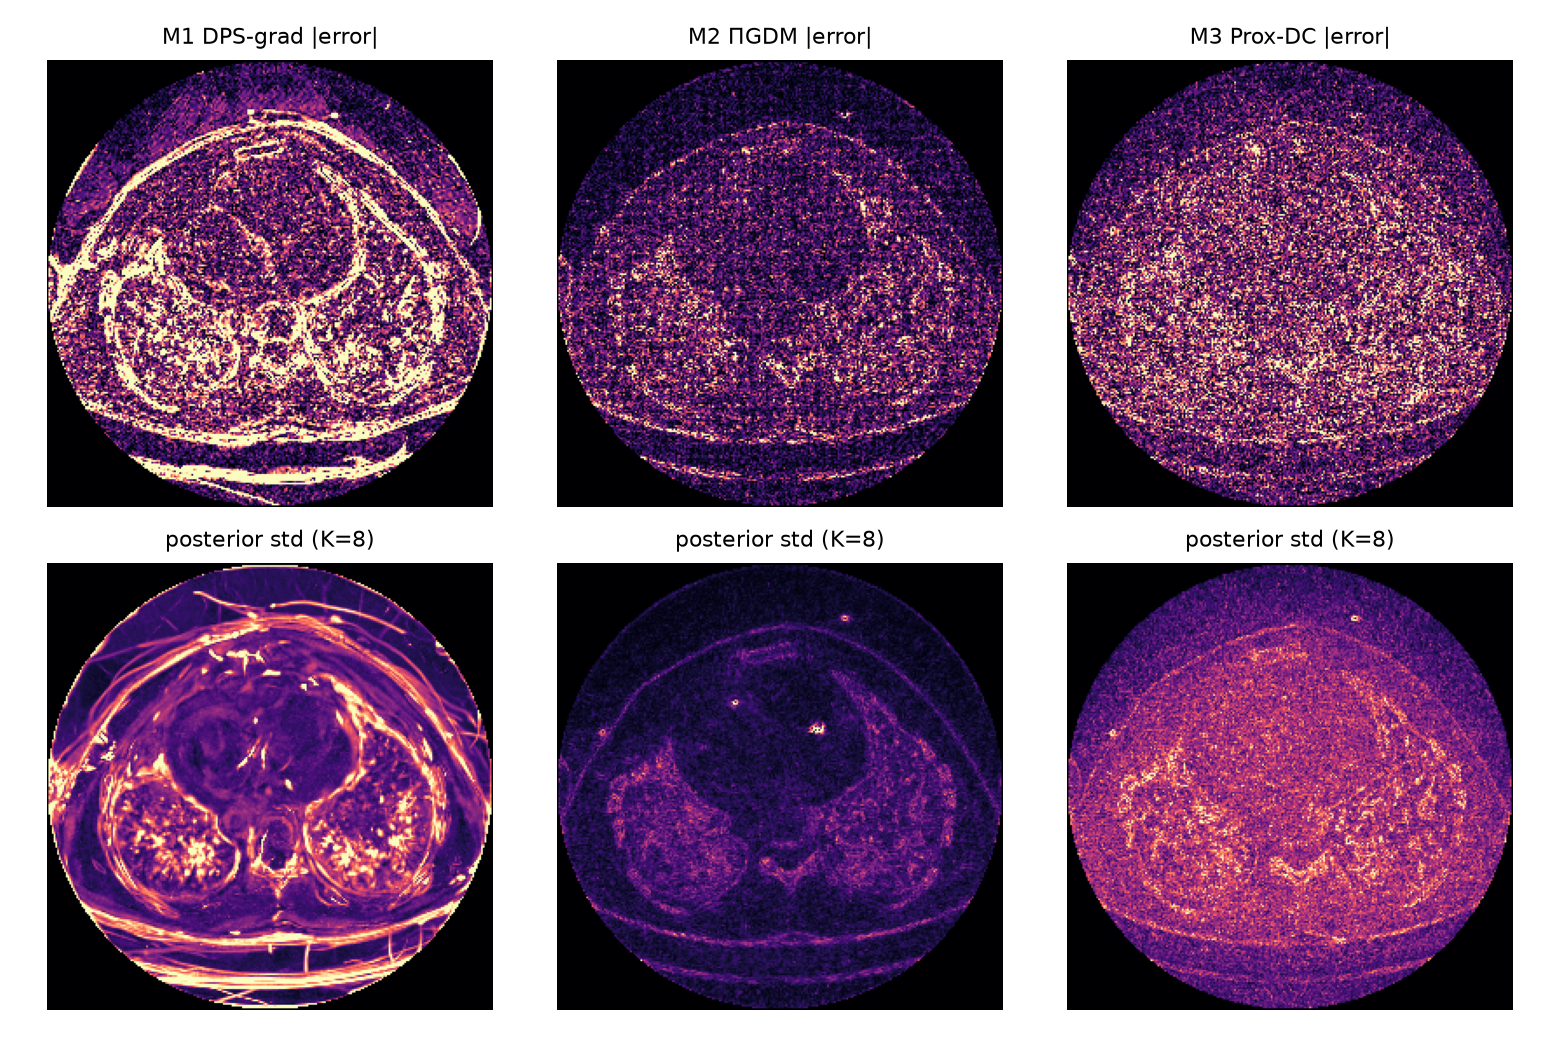
\includegraphics[width=0.85\linewidth]{figures/uncertainty.png}
\caption{单个样本的绝对误差（上）与 8 个样本的后验标准差（下），60 视角，与图~\ref{fig:qual} 为同一切片。M1 的误差与不确定性
沿解剖结构分布（它生成了不同的结构）；M2 的不确定性小且集中在边缘；M3 的不确定性呈噪声状。}
\label{fig:unc}
\end{figure}

\paragraph{步数效率。}
图~\ref{fig:nfe} 在 60 视角下改变 NFE。M3 在 20 步时已达 36.2\,dB（200 张切片 36 秒），步数增加后反而略有\emph{下降}（100 步时
35.7\,dB），这与"硬投影被更频繁地施加在含噪中间估计上"相符。M2 随步数增加而提升（34.3$\to$37.4\,dB），100 步时最好；M1 提升最多
（19.1$\to$28.1\,dB），但即使 100 步仍低于 FBP。

\begin{figure}[t]
\centering
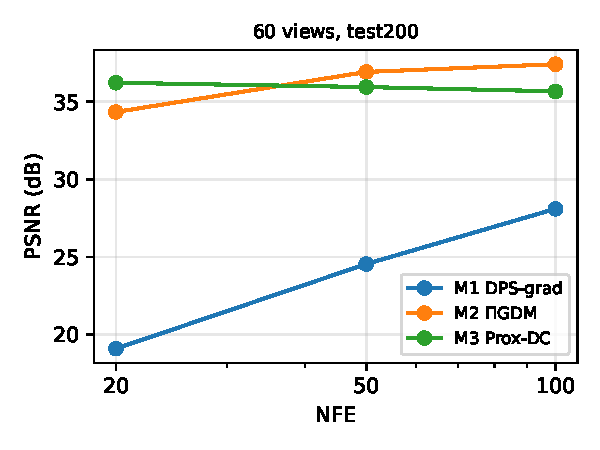
\includegraphics[width=0.45\linewidth]{figures/nfe.pdf}
\caption{60 视角下 PSNR 随 NFE 的变化（test200），引导强度固定为 NFE 50 时选定的值。得益于 $\Delta t$ 缩放，积分后的总引导量
在各 NFE 下相同。}
\label{fig:nfe}
\end{figure}

\paragraph{梯度引导为何在流 ODE 上失效。}
在一次初步测量中（4 张验证切片，60 视角，4 万步中间权重，NFE 20），M1 引导梯度的均方根在 $t{=}0$ 时约为 1.9，而 $t\ge 0.2$ 时只有
0.03--0.07，下降约 60 倍，我们将其归因于纯噪声处网络雅可比很大；用最终权重的测量留待下一版。因此单一的 $\zeta$ 要么在第一步就把
样本推离数据流形，要么在之后太弱：$t_s{=}0$ 时最好的验证 PSNR 只有 13.8\,dB（16 张，NFE 20），必须把引导推迟到
$t_s{=}0.2$--$0.4$（图~\ref{fig:tune}）。即便调过参，M1 在 30、60、90 视角下都饱和在约 24.5\,dB（表~\ref{tab:main}）。使用残差
\emph{范数}的梯度时，步长不随 $\|\bm r\|$ 缩放，因而无法随一致性改善而减小；我们推测正是这一点加上恒定的 $\zeta$（而非 ODE 本身）
造成了与视角数无关的平台。随时间变化的引导权重~\cite{moroy2026guidanceweights} 是自然的改进方向，留待后续工作。其样本只达到粗略
一致（DC 约 3.8\%，与 FBP 相当，是 M2/M3 的十倍以上），并会产生解剖结构幻觉（图~\ref{fig:qual}、图~\ref{fig:unc}）。修正项随残差
消失的 M2 与 M3 没有这种表现。

\begin{figure}[t]
\centering
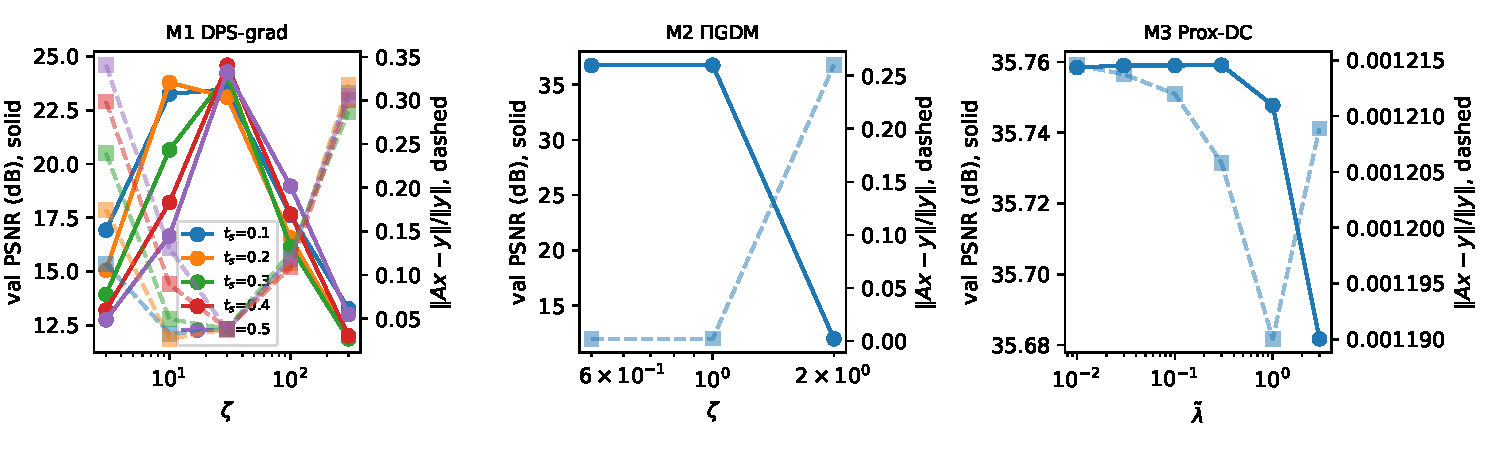
\includegraphics[width=\linewidth]{figures/tuning.pdf}
\caption{60 视角下验证 PSNR（实线）与数据一致性（虚线）随引导强度的变化。M1：每个起始时刻 $t_s$ 一条曲线；M2 在 $\zeta{=}2$ 时发散；
M3 在两个数量级的 $\tilde\lambda$ 范围内都不敏感。}
\label{fig:tune}
\end{figure}

\paragraph{低剂量。}
存在 Poisson 噪声时情况不同。$I_0{=}10^5$ 时监督的 FBPConvNet 最好（35.3\,dB），比 M2 高 2.2\,dB（CI $[1.86,2.49]$），比 M3 高 4.7\,dB；
M3 需要很强的近端权重（$\tilde\lambda{=}30$）才不会把噪声带进图像。在光子饥饿的 $I_0{=}10^4$ 下，直接沿用 $I_0{=}10^5$ 的强度、不重新调参，
排名倒转：FBP 18.0、M3 20.6、M2 22.5、M1 24.5\,dB。M1 最稳健，可能正是因为它对数据利用最少。我们有意没有给 M2 和 M3 噪声模型
（$\sigma_y{=}0$，无加权最小二乘），这在 Poisson 噪声下对它们不利，而 FBPConvNet 会隐式地学到噪声统计；重新调参或引入噪声模型能否
弥补差距，仍是开放问题。

\paragraph{敏感性。}
M3 最容易部署：在 $\tilde\lambda\in[0.01,1]$ 范围内，验证 PSNR 变化不到 0.1\,dB（图~\ref{fig:tune}）；在无噪设置下它实际上相当于硬投影。
M2 有明确的稳定性上限（稀疏视角下 $\zeta{=}2$ 即发散），M1 则需要二维搜索。

\FloatBarrier
\section{讨论与局限}
对于无噪稀疏视角 CT 中的流匹配先验，本文结果支持修正项随残差消失的规则：中等 NFE 下单样本最好的是伪逆引导，少步采样和后验均值
最好的是近端一致性。从扩散 SDE 移植过来、使用单位范数步长的梯度引导，即使调好单位和起始时刻，在 ODE 上也没有竞争力。存在光子噪声时，
两种一致性规则都需要显式噪声模型或按剂量调参，才能赶上监督网络。

本研究有明确的局限。前向模型是作用在重建体数据上的仿真平行束投影，因此算子完全已知，训练与测试一致；扇束 / 锥束几何、算子失配
以及真实投影数据（如 Mayo LDCT）都没有涉及。真值体数据本身包含含噪的临床扫描，这限制了可达到的 PSNR，也会惩罚去噪行为。引导强度
对每种噪声情形只调一次，再迁移到不同视角数和剂量，这对最优值容易迁移的规则有利；我们把这视为测量内容的一部分。监督基线的样本遍历数
约为先验的 1/25，因此其数字是下界。先验是二维的，不保证层间一致性~\cite{chung2023diffusionmbir,song2024diffusionblend}；M1 的轨迹
分析使用的是中间权重；后验均值结果只用了 $K{=}8$（60 视角）和 $K{=}4$（30 视角）个样本。

\section*{代码与数据}
代码、配置文件、逐图指标以及各划分的病人列表公开于 \url{https://github.com/ZeroDevi1/flow-ct-guidance}。数据为公开的
TotalSegmentator v2.0.1（CC-BY-4.0）。

\section*{致谢}
本文的实验代码、实验执行与论文初稿借助了 AI 编程助手（Claude，Anthropic）完成。全部结果与文字均经作者核查，作者对内容负全部责任。

\bibliographystyle{unsrtnat}
\bibliography{references}
\end{document}
